\documentclass[a4paper,11pt]{article}
% --------------------------------------------------------------------------------------------------------> PACKAGES <--- %
\usepackage[frenchb]{babel}
\usepackage[utf8]{inputenc}
\usepackage{url}
\usepackage{graphicx}
\usepackage{tabularx}
\usepackage{eurosym}
%\usepackage{epsfig}
\usepackage{bibtopic}
\usepackage{comment}
\usepackage{tikz}
\usepackage{amsmath}

% --------------------------------------------------------------------------------------------------------> META DATAS <--- %
\usepackage[
  colorlinks=false,
  pdfborder={0 0 0},
  pdfauthor={Emmanuel Roubin},
  pdftitle={Roubin Emmanuel | Curriculum Vitae},
  pdfsubject={Curriculum Vitae},
  pdfkeywords={Materiaux a matrice cimentaire, Milieux heterogenes, Modele morphologique, Modelisation multi-echelles, Embedded Finite Element Method},
  pdfproducer={LaTeX with hyperref package},
  pdfcreator={pdflatex, bibtex}
]{hyperref}

% --------------------------------------------------------------------------------------------------------> MARGIN <--- %
\pagestyle{empty}
\usepackage{vmargin}
\setmarginsrb{1.cm}{1.5cm}{1.5cm}{1.cm}{0cm}{0cm}{0cm}{0cm}

% --------------------------------------------------------------------------------------------------------> TITLE <--- %
\newcommand{\titre}[1]{
  \begin{center}
    \rule{0.4\textwidth}{0.5pt}
    \par\vspace{0.1cm}
    \textsc{\large #1}
    \par\vspace{-0.2cm}
    \par\noindent\rule{0.4\textwidth}{0.5pt}
  \end{center}
}

% --------------------------------------------------------------------------------------------------------> BEGIN DOCUMENTS <--- %
\begin{document}
\begin{center} \par\textsc{\huge Curriculum Vit\ae} \end{center}
\begin{minipage}{0.7\linewidth}
  \begin{flushleft}
    \LARGE Emmanuel ROUBIN \normalsize  \vspace{0.1cm} \\
    \large Maître de conférence à l'Université Grenoble Alpes \normalsize\\\vspace{0.2cm}
    IUT 1 Département GCCD --- Laboratoire 3SR UMR 5521\\
    \href{mailto:emmanuel.roubin@3sr-grenoble.fr}{emmanuel.roubin@3sr-grenoble.fr}\\\vspace{0.2cm}
    15/03/1986 (31 ans)
  \end{flushleft}
\end{minipage}
\hfill
\begin{minipage}{4cm}
  %\centering \fbox{\href{http://perso.crans.org/roubin}{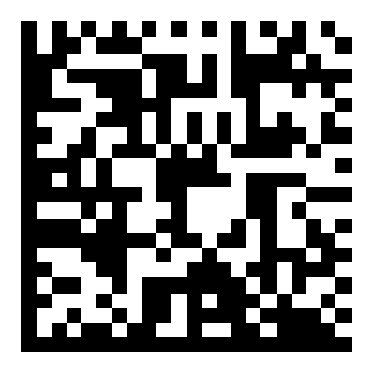
\includegraphics[width=3cm]{img/flashcode.eps}{}}}\\\vspace{0.1cm} \footnotesize\href{http://perso.crans.org/roubin}{perso.crans.org/roubin}
  \centering
  \fbox{\href{http://perso.crans.org/roubin}{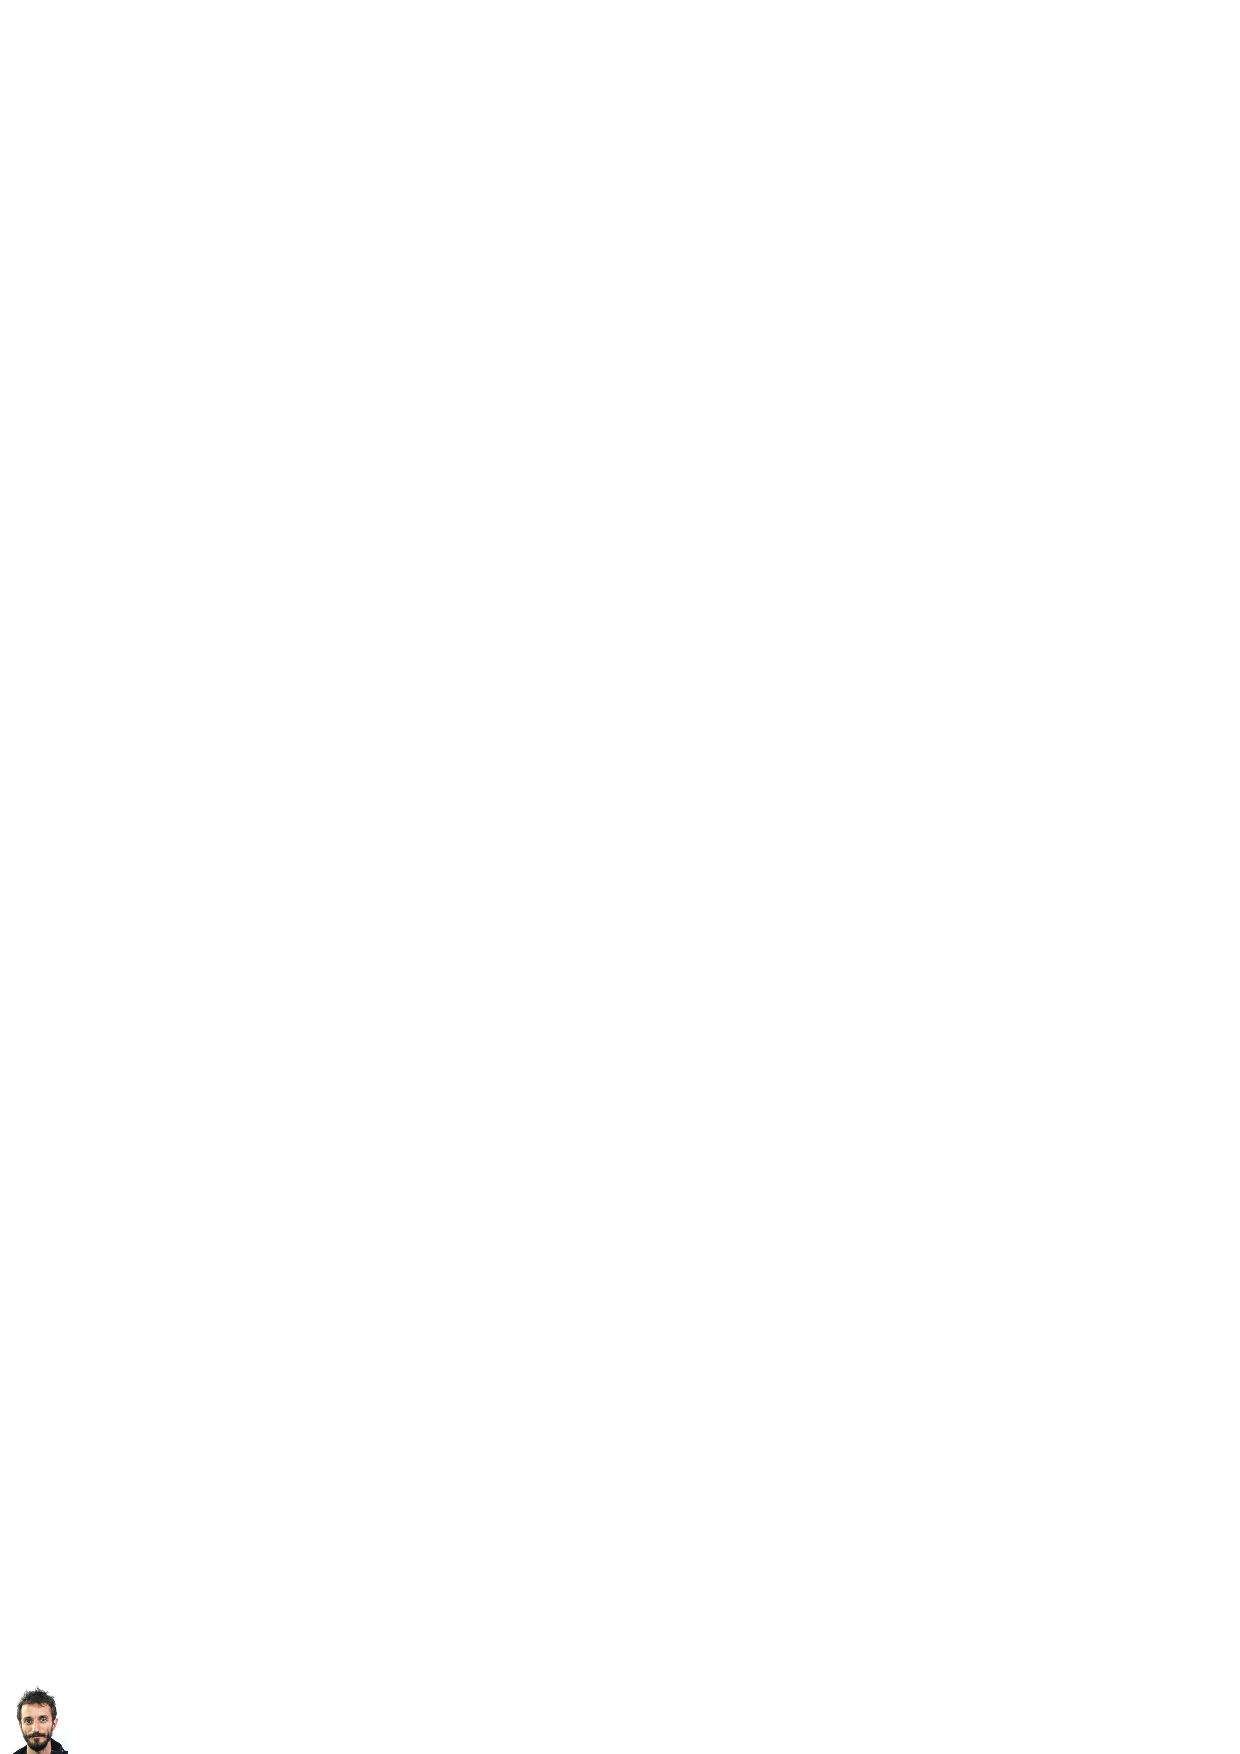
\includegraphics[width=2cm]{img/id.png}{}}} \\ \vspace{0.1cm}
  \footnotesize\href{http://perso.crans.org/roubin}{perso.crans.org/roubin}
\end{minipage}
\vfill
%\begin{center}
%  \textsc{Profil : Chercheur en Génie Civil / Numéricien / Ancien moniteur de l'ENS Cachan}
%\end{center}

% --------------------------------------------------------------------------------------------------------> PARCOURS <--- %
\titre{Parcours}
\begin{tabular}{p{0.2\textwidth}p{0.75\textwidth}}
    Depuis Sept. 2015 & \textbf{Maître de conférence} de l'Université Grenoble Alpes (UGA) à l'IUT1 GCCD. Rattaché au laboratoire 3SR (UMR 5521).\hfill \raisebox{-0.2cm}{\includegraphics[height=0.6cm]{img/3sr.png}\includegraphics[height=0.6cm]{img/iut1_h.png}}\\
    0ct. 2013 - juin 2015 & \textbf{Post-doctorant} à l'International Center for Numerical Methods in Engineering (CIMNE), UPC Barcelone (Espagne), avec le Professeur X. Oliver.\hfill \raisebox{-0.2cm}{\includegraphics[height=0.6cm]{img/cimne.png}}\\
    Sept. 2010 - oct. 2013 & \textbf{Doctorant} au Laboratoire de Mécanique et Technologie (LMT-Cachan, UMR 8535) sous la direction de Jean-Baptiste Colliat.\hfill \raisebox{-0.2cm}{\includegraphics[height=0.6cm]{img/lmt.jpg}}\\
    Sept. 2006 - juin 2010 & \textbf{Élève normalien} à l'ENS~Cachan. Diplôme M2 Génie Civil.\hfill \raisebox{-0.2cm}{\includegraphics[height=0.6cm]{img/cachan.png}}
\end{tabular}
\vfill

% --------------------------------------------------------------------------------------------------------> RECHERCHE <--- %
\titre{Activités de recherche}
\begin{itemize}
  \item[\textbf{Thématiques}] : Modélisation numérique du comportement des bétons aux échelles fines
    \begin{itemize}
    \item Modélisation du caractère aléatoire de la \textbf{morphologie} (inclusions, porosité, percolation)
    \item Analyse \textbf{multi-échelles} et \textbf{multi-physiques}
    \item Caracétisation de champs 3D issues d'{\bf images tomopgraphiques} d'essais mécaniques ({\bf DVC}).
    \item Modélisation de la \textbf{fissuration} et procédures de \textbf{réduction de modèles}
    \end{itemize}
  \item[\textbf{Projets}] : ANR MOSAIC (Lille, LML, 2015-) portée J.-B Colliat, ERC COMP-DES-MAT (Barcelone, CIMNE, 2013-2015) porté par X. Oliver.
  \item[\textbf{Encadrements de thèses}] : Olga Stamati (Grenoble, 3SR, 2016-), Yue Sun (Lille, LML, 2016-), Paul Hauseux (Lille, LML, 2012-2015)
%   \item[\textbf{Encadrements de stage de Master}] : Mateusz Bogdan (Cachan, LMT, 2011), Hala Damerji (Grenoble, 3SR, 2016), Olga Stamati (Grenoble, 3SR, 2016)
  %\item Thèse Alexis Vallade (LML, 2012-2016) : \textit{``Modélisation multi-échelle du gaz de schiste. Influence de la microstructure sur les propriétés macroscopiques et le procesus de fracturation.''}
  %\item Stage M2 Olga Stamati (3SR, 2016) : \textit{From x-ray tomography to FE simulation of cementitious materials: Making the link with quantitative image analysis}
  %\item Stage M2 Hala Damerji (3SR, 2016) : \textit{Mesoscale modeling of concrete failure under dynamic loading: Application to spalling test}
  %\item Stage M2 Mateusz Bogdan (LMT, 2011) : \textit{Modèle morphologique d'hydratation de matrices cimentaires} 
  \item[\textbf{Principales contributions}] :
    \NoAutoSpaceBeforeFDP
    \begin{btSect}[bibperso/chrono]{bibperso/Published_top_five}
      \btPrintAll
    \end{btSect}
    \AutoSpaceBeforeFDP
  \item[\textbf{Principales conférences}] : WCCM (Espagne, 2014), WCCM (Brésil, 2012), COMPLAS (Espagne, 2011)
\end{itemize}
\vfill

% --------------------------------------------------------------------------------------------------------> COMPETENCES <--- %
\titre{Enseignements}
\begin{itemize}
  \item[\bf Direction des études] : $1^\text{ère}$ et $2^\text{ème}$ années ($\approx 250$ étudiants) depuis septembre 2016.
  \item[\bf Enseignements (IUT)] : géotechnique et mathématiques depuis septembre 2015.
  \item[\bf Monitorat (M1/M2)] : Mécanique des milieux continus, méthodes numériques, probabilités, mécanique probabiliste entre septembre 2010 et juin 2013
\end{itemize}
\vfill
\empty
\end{document}
